\section{Stream Summarization}

Stream data has become more and more important since the rise of the Internet of
Things. Devices in IoT communicate using stream data. Stream data is transmitted
at high speed, and short intervals. Hardware also has limited storage, so
stream data may never be reviewed if the system does not process it immediately. Some
stream summarization techniques have been researched and proposed to address issues
related to high data volume and
velocity. We introduce several stream summarization techniques in this section.

\subsection{Overview of Stream Problems and Algorithms}
Most data stream analysis algorithms rely on data reduction and synopsis
construction techniques to compute approximate solutions that work with limited
storage and in constant time. In this chapter, we introduce the following data
reduction and synopsis construction techniques:
\begin{quote}
\begin{itemize}
    \item  \textbf{Sampling} captures a sub-sample of a data stream that represents
    the entire data stream. It can be used to extract essential
    characteristics of a data stream~\cite{kejariwal2015real}.
    
    \item \textbf{Filtering} eliminates useless or unwanted data points from a
    stream. We can only capture the data which we are interested in. An
    example is filtering spam email.
    
    \item \textbf{Sliding windows} maintain a window that moves with new data
    coming, it ensures the analysis and statistics using fresh data. It is also 
    often used to record data in given bounded memory.

    \item \textbf{Frequency Moments} show the characteristics of the stream.
    Moments involve the distribution of frequencies of different elements in
    the stream. 

    \item \textbf{Clustering} separates the data points into different groups.
    It makes sure that the points in one
    group as similar as possible, the points in different group as different as
    possible. For instance, they can be applied to problems such as the k-median 
    problem \TG{k-median is a clustering technique, not an application}. 

\end{itemize}
\end{quote}

For each problem in streaming research, there are many algorithms to solve or
estimate it. The remainder of this chapter presents certain algorithms used in
specific streaming analysis problems.

\subsection{Sampling}

When the data is huge and we cannot save it into working storage, we could extract
sampling data from the whole data stream. Estimating the result base on fraction
of the sample and whole data.
\english{But there are some trick in it}. There is a
instance from~\cite{leskovec2014mining}: to query ``What fraction of the typical
user's queries were repeated over the past month?''. The common idea is to
extract 1/10 of data from the whole stream, each data has 10\% probability be
selected. Assume a user issues N search queries in past month, only D search
queries issue twice, other queries once. The fraction of queries that appear twice after sampling
is$\frac{D}{100}$, because the probability of a data point to appear twice in sample
is$\frac{1}{10}*\frac{1}{10}$(first time \english{appear} is $\frac{1}{10}$, the second
\english{appear} also needs $\frac{1}{10})$. $\frac{18D}{100}$ repeated queries appear only
once in sample($2*\frac{1}{10}*\frac{9}{10}$). The correct answer is
$\frac{D}{N}$, while the answer we obtain after sampling is:
\begin{equation*}
    \frac{\frac{D}{100}}{\frac{N-D}{10}+\frac{18D}{100}+\frac{D}{100}} = \frac{D}{10N+9D}
\end{equation*}
Thus, the estimated obtained from the sampled data is incorrect.

Another idea is to extract the queries from 1/10 of users. Using a hash
function (result 0-9 \TG{explain more}), the queries are accepted for the
sample, if the user id hashes to 0. In this instance, we take $user$ as the
key. 

So, in the general sampling problem, to take a $\frac{a}{b}$ size sample
from the whole stream, we can hash the key value to $b$ buckets, and accept
data for sample while the hash value less than
$a$~\cite{leskovec2014mining}.

In practice, sampling can help save energy on connected objects. For
instance, when querying a question on stream, we can estimate the result
after sampling from whole stream. We need less communication with objects,
because we need only a part of whole stream to estimate result.  

\subsection{Filtering}

Sometimes, we are interested only in particular elements in the stream. For
instance, some connected sensor objects send longitude and
latitude stream data to client side. In this case, if we are only interested by
the data from specific longitudes and latitudes, filtering stream is needed.
In another example, we are receiving a list of email addresses which include lots
of spam. Therefore, we need to filter the stream and focus on the non-spam
addresses. Assume we have list of email addresses that is too large to be stored
in main memory. The technique knows as \textbf{Bloom
filtering}~\cite{bloom1970space} could be used. 
\TG{Avoid bold text}

\paragraph{Bloom Filter}

The Bloom filter uses $n$ bits for filtering, $m$ non-spam email
addresses in list $S$, and $k$ hash functions. Each hash function maps an email
address into $n$ buckets. An array of $n$ bits is initialized as follows: 
\begin{enumerate}
  \item Initialize an array of bits $N$ by setting 0's in $n$ bits.
  
  \item For each email address in $S$, hash the address with all
  hash functions and change the value of corresponding bit to 1 based on hash
  result.
\end{enumerate}

\TG{Refer to the MMDS book more explicitly throughout this chapter, as
most references are taken from it.}

After initialization, each new coming stream data will be filtered by using the
array of bits $N$ and $k$ hash functions. When a new stream element comes,
we can get a bits result from those hash functions. \english{Adding this
data for sample if the result are all 1's, otherwise filtering it.
\TG{``ing'' is not the right form, please review grammar (I fixed many
occurrences before)}}  However, email addresses that are not in $S$ might
pass the filter too, and be selected in the sample. We would like to calculate
the probability of a spam to be selected in the sample. Obviously, the spam
is harder to pass, if the fraction of 0 bits in bit array $n$ \TG{verb is
missing}. During the bit array initialization stage, we have $m$ emails in
$S$, and $k$ hash functions. For each email in $S$, suppose hash result
corresponds to target bit. The probability that a hash result hits a given
bit is $\frac{1}{n}$. Conversely, the probability that a hash result does
not hit a given bit is $\frac{n-1}{n}$. Because we have $k$ hash functions,
the probability that
one email does not hit a given bit is $(\frac{n-1}{n})^k$. After hashing $m$ emails,
the probability that a bit in bit array still remains 0 is
$(\frac{n-1}{n})^{km}$, which equals $(1-\frac{1}{n})^{n(\frac{km}{n})}$. It
is approximated by $e^{-\frac{km}{n}}$, using the approximation
$(1-\epsilon)^\frac{1}{\epsilon} = \frac{1}{e}$. For a new coming spam stream
data, the probability that it is selected for sample is
$(1-e^{-\frac{km}{n}})^k$, which is the false positive rate of the filter.

\subsection{Frequency Moments}

Alon et al.~\cite{alon1999space} introduced the frequency moments in 1996.
Frequency moments are important statistics for large size data. $F_0$ is
the number of distinct elements in data. $F_1$ is the number of elements in
the data. $F_2$ presents the surprise index of data stream. In general,
$F_k$ represents the degree of skew in the data. Assume A =
$(a_1,a_2,...,a_m)$ is a sequence of elements, and each element $a_j \in
\llbracket1, n\rrbracket$. $m_i$ denotes the number that the element $i$
appears in A, $i \in \llbracket1, n\rrbracket$ \TG{Revise, this is wrong.}.
Generally, for $k\geqslant0$, the $k^{th}$ frequency moment of a set of
frequencies \textbf{m} \TG{why bold?} is defined as: 
\begin{equation*}
F_k(m) = \sum_{i=1}^n m_i^k     
\end{equation*}
In the rest of this section, we present algorithms to estimate frequency moments. 

\subsubsection{First Moment (Distinct Elements in Stream)}

From the definition of frequency moments, the first moment represents
the number of distinct elements in the data stream, also known as
\texttt{Cardinality}. To count the number of distinct elements in a stream, the
naive method is to store the elements in a set. When a element comes, we
check whether this element is already present, if not we add it to the set.
A traditional method to store this element uses a B-Tree, because of
its good efficiency to search and insert elements. But a B-Tree requires more
storage space, and it is less efficient for merging when the data sets is large. Using
bitmap is a another traditional method, hashing every element into a bit array
by hash function. If value of bit is 1, then the element is already presented,
otherwise change the bit from 0 to 1. Bitmap is good at merging (just using OR
operation), and only need Ns bits for element x $\in \{1...n\}$. But if the N is
large or undefined, bitmap is not good choice \TG{why?}.

\paragraph{Linear Counting Algorithm}

The linear counting method was introduced in~\cite{whang1990linear} by Whang et
al, to estimate the number of distinct elements in stream. Assume a hash function
can hash elements into $m$ buckets. A bit array of $m$ size is maintained,
updating value of bit into 1, if the hash result hits the corresponding buckets.
We suppose the number of bits set to 0 in bit array is $u$. Therefore, the number
of distinct elements is estimated by $\hat{n} = -mlog\frac{u}{m}$. This is
because the probability that the $j^{th}$ bit in bit array remains 0, referred
to as $P(A_j)$, is $(1-\frac{1}{m})^n$ (assume the result from hash function is
independent uniform distribution). The expectation of $u$ 0's bits is $E(u)$ =
$\sum_{j=1}^{m} P(A_j)$ = $m(1-\frac{1}{m})^n$ =
$m((1+\frac{1}{-m})^{-m})^{-\frac{n}{m}}$, which approximates to
$me^{-\frac{n}{m}}$. \TG{Use \textbackslash left( and \textbackslash right) for parentheses.}
According to above, $n$ = $-m\log{\frac{E(u)}{m}}$. This method needs large
enough memory to save bit array. To reduce collisions, the size of
the bit array must be far greater
than the number of distinct elements in stream.

\paragraph{Flajolet-Martin Algorithm}

Flajolet and Martin proposed an algorithm~\cite{flajolet1985probabilistic} to
estimate cardinality. This algorithm applies a hash function $h$ to hash each
element of the stream into a bit-string. For each bit-string (hash-values), we denote
by $tail\ length$ the number of 0's at the end of bit-string. Assume $R$ is the
maximum number of the $tail\ length$ in the stream. Then we can estimate the
number of distinct elements in stream with
$2^R$~\cite{flajolet1985probabilistic}. This is because the probability that a
bit-string from $h(a)$ has at least $r$ 0's in then end is $2^{-r}$. The
probability that no bit-string has $tail\ length \geqslant r$ after hashing all
elements in the stream is $(1-2^{-r})^n$ = $((1-2^{-r})^{2^r})^{n2^{-r}}$ =
$e^{-n2^{-r}}$, assuming there are $n$ distinct elements in the
stream~\cite{leskovec2014mining}. Thus, $1-e^{-n2^{-r}}$ is the probability that
there is one or more than one $tail\ length$ of bit-string at least $r$, refer
to as $P(tl \geqslant r)$. From above we can know, $P(tl \geqslant r) \approx
0$, if $n \ll 2^r$. Conversely, if $n \gg 2^r$ then $P(tl \geqslant r) \approx 1$. So
$2^{R}$ \english{can be a evaluation for cardinality of stream, which unlike causes big
error}.

The accuracy of this Algorithm is not outstanding, because of growth with a base
2 index. But we only need to record the maximum $tail\ length$ in main
memory~\cite{leskovec2014mining}. Assume a stream has $n$ distinct elements. It
needs $O(\log n)$ bits to record bit-string ($n$ different results). Because $R$
is lower or equal to the size of the bit-string, $O(\log\log n)$ bits is enough to
record longest $tail\ length$ and to estimate the number of distinct elements. 
\paragraph{Loglog Counting Algorithm}

Loglog Counting Algorithm~\cite{durand2003loglog} is similar to
Flajolet-Martin Algorithm. But this algorithm estimates the cardinality of
stream by using the leftmost 1-bit position of bit-string rather than $tail \
length$ which used by Flajolet-Martin Algorithm. The leftmost 1-bit position of
a bit-string $i$, refer to as $L_i$. The probability of all $L_i \leq k$ is
$(1-2^{-k})^n$. Thus, the probability that at least one $L_i \geqslant k$ is
$1-e^{-n2^{-k}}$, where $n$ is the number of bit-strings. In order to reduce
estimate error, Loglog counting separates hash results into $m$ buckets and
$m$=$2^b$~\cite{durand2003loglog}. The first $b$ bits in bit-string is the index
of the buckets. The rest bits in bit-string are used for finding leftmost 1-bit
position. Assume $M_j$ indicates the maximum leftmost 1-bit position among
bit-strings in the $j$ bucket. Thus, we estimate the number of distinct elements
by $\hat{n}$ = $2^{-\frac{\sum M_j}{m}}$~\cite{durand2003loglog}. Loglog
counting Algorithm needs $O(m \log\log(\frac{N}{m}))$ space complexity, where N is
the number of distinct elements in the stream (the number of the hash results), and m is
the number of buckets. 

\paragraph{HyperLoglog Counting Algorithm}

HyperLoglog Counting Algorithm~\cite{flajolet2007hyperloglog} is an improvement
of Loglog Counting Algorithm. The geometric mean used by Loglog Counting
is very sensitive to discrete values, and the buckets might by empty if the
number of elements in the stream is small~\cite{flajolet2007hyperloglog}. Thus,
HyperLoglog Counting Algorithm uses harmonic mean instead of geometric mean.
\english{Thus, The estimate of cardinality of stream shell be obtain by} $\frac{\alpha_m
m^2 }{\sum 2^{-M_i}}$ with $\alpha_m$ = $(m
\int_0^\infty(\log_2(\frac{2+u}{1+u}))^m\ du)^{-1}$ , where $M_i$ expresses the
maximum leftmost 1-bit position among bit-strings in the $i$
bucket~\cite{flajolet2007hyperloglog}.

\subsection{Second Moment $F_2$}

\paragraph{Alon-Matias-Szegedy Sketch}
Alon, Matias and Szegedy~\cite{alon1999space} proposed AMS sketch to solve this
problem \TG{which problem?}. Now, let us assume that we have $d$ hash functions $h_1$, ..., $h_d$
that hash elements into \{1, 2, ..., $w$\}. $d$ extra 4-wise independent hash
functions $g_1$, ..., $g_d$ : $\{1...U\}\rightarrow \{-1, 1\}$. One AMS sketch
$Z$ maintains a $d$*$w$ matrix. Each element $e$ from stream is mapped to an
entry based on the hash function $h_i(e)$ for each row in the matrix. After
mapping elements with $h$ functions, each changed entry $Z[i][j]$ is updated by
$Z[i][j]$ += $g_i(e)*c$, where $c$ is update weight which can be positive or
negative~\cite{garofalakis2016data}. To estimate $F_2$, we can process
\english{estimation from each row $j$, it refer to as $\sum_{k=1}^w Z[j][k]^2$, and
obtain the median of these estimates as final result}.

\subsection{High-Order Moments $F_{k>2}$}
\paragraph{Count-Min sketch}
The Count-Min sketch~\cite{cormode2005improved} was introduced to solve
$F_\infty$ and frequency items problems. It maintains a matrix, referred  as
$CM$, of $w \times d$ size which has a counter in each cell. Applying $d$ pairwise
independent hash function $h_1$, ..., $h_d$ : $\{1...m\} \rightarrow \{1...w\}$,
the counter in each row shell \TG{What is a row shell?} is incremented when a new element $e$
arrives~\cite{garofalakis2016data}. \english{e.g. In} row $j$, the counter
$CM[j][h_j(e)]$ is incremented. We can estimate the frequency of element $e$ with
$\hat{n}_e = \min_{j=1}^d CM[j][h_j(e)]$, thereby estimating higher-order
moments~\cite{cormode2005improved}.


\TG{You review a lot of algorithms that won't be used in your contribution.
I think you could summarize some of the text in this section, in particular counting
algorithms.}

\subsection{Sliding Window}

The sliding window model was addressed by Datar et
al.~\cite{datar2002maintaining} \TG{A model is not ``addressed''}. A
sliding window may contain the most recent $n$ elements of stream, or it
can contain all the elements within specific time period $t$, e.g., one
hour or one day~\cite{leskovec2014mining}. The sliding window model has
been used by many algorithms. We introduces two of them below.

\subsubsection{Sliding HyperLoglog Algorithm}

Sliding HyperLoglog Algorithm is proposed in~\cite{chabchoub2010sliding},
adapting the HyperLoglog algorithm by maintaining some additional time
information. The purpose of this algorithm is to estimate the number of distinct
elements in last $w$ units of time, $w$ smaller than the window size
$W$~\cite{chabchoub2010sliding}. \english{Representing the $L_i$(the position of leftmost
1-bit) by a pair $<t_i, L_i>$, where $t_i$ is the arrival timestamp of
element~\cite{chabchoub2010sliding}, is applied for adding time information}.
\english{There is a list to store pairs in each bucket, which prefer to as
LFPM(\emph{List of Future Possible Maxima})}. \english{Once a new pair $<t_k, L_k>$
arrives, at first we delete old data where $t_i < t_k - W$ where $W$ is the
window size, and delete all data where $L_i \leq L_k$, finally add this new pair
into LFPM of corresponding bucket~\cite{chabchoub2010sliding}. To answer a
request "How many distinct elements during $w$ units of time." at time $t$,
$M_i$, the biggest $L_i$ in each bucket is computed for estimation. Sliding
HyperLoglog gives the same estimate with applying HyperLoglog on the stream
during $[t-w, t]$ period. But It needs more memory usage.}

\subsubsection{LRU-LC Algorithm}

LRU-LC sketch~\cite{shan2016lru} adapts Linear counting sketch to sliding window
model. It applies the well-known memory page replacement algorithm, least
recently used replacement policy~\cite{o1993lru} (LRU) to evict stale
information in time order~\cite{shan2016lru}. To update \english{the aging degree of
information from the sketch}, the entry array $V$ is used instead of bit array
which LC retains. Each entry consists of backward pointer (bp), forward
pointer (fp) and \english{time different} \TG{time difference?} between two adjacent items ($\bigtriangleup t$),
$\bigtriangleup t_i$ = $t_i - t_{i-1}$. \english{It is marked as two state}: $active$ (\english{be
hit during last $W$ unites of time}) and $inactive$ \TG{There is always a space before an opening
parenthesis, and after a closing one} (\english{stale or be not hit}), and
grouped into different parts of LRU-LC. All active entries constitute linked
queue refer to as LRU queue, and are sorted in order of the last time it is hit,
as figure~\ref{fig:LRU-LC}. Assume the LRU queue has $k$ entries, thus, the
aging degree of an entry $V[i]$ in LRU queue shell be calculated as:
\begin{equation*}
   D_{aging}[i] = W-\sum_{j=i}^{k}\bigtriangleup t_j
\end{equation*}

Where $D_{aging}[i]$ indicates the aging degree of the entry $V[i]$, $W$ is the
window size~\cite{shan2016lru} and $\bigtriangleup t_j$ is the component
$\bigtriangleup t$ in the entries of LRU queue which behind $V[i]$. The active
entries shell be removed and sent into inactive group, if its aging degree
equals 0. We shows algorithm of LRU-LC in Algorithm~\ref{algo:LRU-LC}. LRU-LC
updates aging degree of entries by decreasing $\bigtriangleup t$ of the first
entry in LRU queue, see line 26-27 in Algorithm~\ref{algo:LRU-LC}. Finally, the
cardinality of the stream over the window $W$(during $W$ units of time) shell be
estimated by $ -mlog\frac{z}{m}$, where $z$ is the number of $inactive$ entries
and $m$ is the size of the array(the number of buckets for hashing).
\TG{This sub-section is very difficult to read, it needs improvement (I stopped half-way).}

\TG{I don't think that the algorithm is necessary here.}

\begin{algorithm}
\caption{Algorithm of LRU-LC}
\label{algo:LRU-LC}
\begin{algorithmic}[1]
\Input
    \Desc{$e_i$}{Element from stream}
    \Desc{$m$}{Size of entry array(number of the entries)}
    \Desc{$V$}{entry array in of LRU-LC}
    \Desc{Q}{LRU queue}
\EndInput
\Output
    \Desc{$z$}{Number of inactive entries}
\EndOutput

\State $index$ = h(e) \Comment{Obtain entry index of entry}
\State $\delta t$ = $e_i.t$ - $e_{i-1}.t$
\If {$V[index]$ is inactive}
    \State $V[index].\bigtriangleup t$ = $\delta t$
    \State Q.append\_back($V[index]$)
    \State $z$ -= 1
\Else \Comment{$V[index]$ is active}
    \If {$V[index]$ == Q.end()} \Comment{Last entry of queue}
        \State $V[index].\bigtriangleup t$ += $\delta t$
    \Else
        \State $v_F$ = $V[index].fp$
        \State $v_B$ = $V[index].bp$
        \State $v_F.bp$ = $V[index.bp]$
        \State $v_B.fp$ = $V[index.fp]$
        \State $v.\bigtriangleup t$ += $V[index].\bigtriangleup t$
        \State Q.append\_back($V[index]$)
    \EndIf
\EndIf
\State $v_{first}$ = Q.first() \Comment{First entry of queue}
\State $v_{first}.\bigtriangleup t$ -= 1
\If{$v_{first}.\bigtriangleup t$ == 0}
    \State Q.remove($v_{first}$)
    \State $z$ += 1
\EndIf
\end{algorithmic}
\end{algorithm}

\begin{figure}
    \centering
    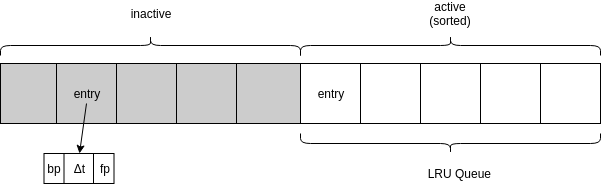
\includegraphics[width=0.8\columnwidth]{figures/LRU-LC.png}
    \caption{Structure of LRU-LC}
    \label{fig:LRU-LC}
\end{figure}

\subsection{Clustering}

\subsubsection{CluStream Framework}

In the paper~\cite{aggarwal2003framework} authors discussed a clustering framework
for evolving data streams. It is called CluStream. This framework
has two components, the Online micro-clustering component is used for storage
of summary statistic in data stream. These information are computed based on
micro-clusters which use \textbf{cluster feature vector}~\cite{zhang1996birch}
to cluster data streams. In online component, pyramidal pattern is used to
store micro-clusters as snapshots in order to acquire summary statistics over
different time horizons. The offline component \english{is designed for analyst}, which
\english{can present quick understanding of the clusters of data streams with the
statistic information from online component and specific input, for example what
time horizon is using for clustering, how many clusters should data stream
be clustering} \TG{Sentence is way too long}. In the offline
macro-clustering component, we can use its \emph{subtractive} property of
the micro-clustering to generate higher level clusters over different time
horizons~\cite{aggarwal2003framework}. \english{For instance, the current clock time
is $t_c$ and the user wishes to find clusters
on a time horizon of length h, then we can find the snapshot in $t_c$ and $(t_c-
h)$ then we can get the clusters with time horizon of length h}. It is not
possible to save snapshots for every moment, so this framework \english{using} pyramidal
time frame to storage snapshots with different orders. The order of a class of
snapshots means that the level of granularity in real
time~\cite{aggarwal2003framework}.
